\documentclass[10pt,aspectratio=169]{beamer}

\usepackage{amsmath}

\usepackage{presento/config/presento}
\usepackage{tikz}
\usetikzlibrary{shadings,shadows,calc,backgrounds,positioning}
\usepackage{tcolorbox}
\usepackage{adjustbox}
\usepackage{bytefield}
\newcommand{\colorbitbox}[3]{%
    \rlap{\bitbox{#2}{\color{#1}\rule{\width}{\height}}}%
    \bitbox{#2}{#3}}
\tcbuselibrary{skins,breakable}

\usepackage{caption}

\usepackage[caption=false]{subfig}
%\usepackage{transparent}
\setbeameroption{show notes}

%\usepackage[backend=bibtex]{biblatex}
\usepackage{natbib}
%\bibliography{bib/myrefs}

\definecolor{darkblue}{HTML}{000099}
\usepackage{listings}
\lstset{
    frameround=fttt,
    language=C,
    numbers=left,
    %stepnumber=5,               % Abstand zwischen den Zeilennummern       
    %numberfirstline=false
    breaklines=true,
    keywordstyle=\color{black}\bfseries, 
    basicstyle=\ttfamily\footnotesize\color{darkblue},
    showstringspaces=false,
    numberstyle=\color{black}
    }
\lstMakeShortInline[columns=fixed]|

% figures
\usepackage {pgf}                                 % includepgf for bitmaps
\usepackage{graphicx}

% Information
\title{Extending Compiler Support for the BrainScaleS Plasticity Processor}
\subtitle{Bachelor's Thesis Presentation}
\author{Arthur Heimbrecht}
\institute{}
\date{\today}

\begin{document}


% Title page
{
\usebackgroundtemplate{
    \tikz[overlay, remember picture]\node[opacity=0.3, inner sep=0, outer sep=0, ] at (current page.center) {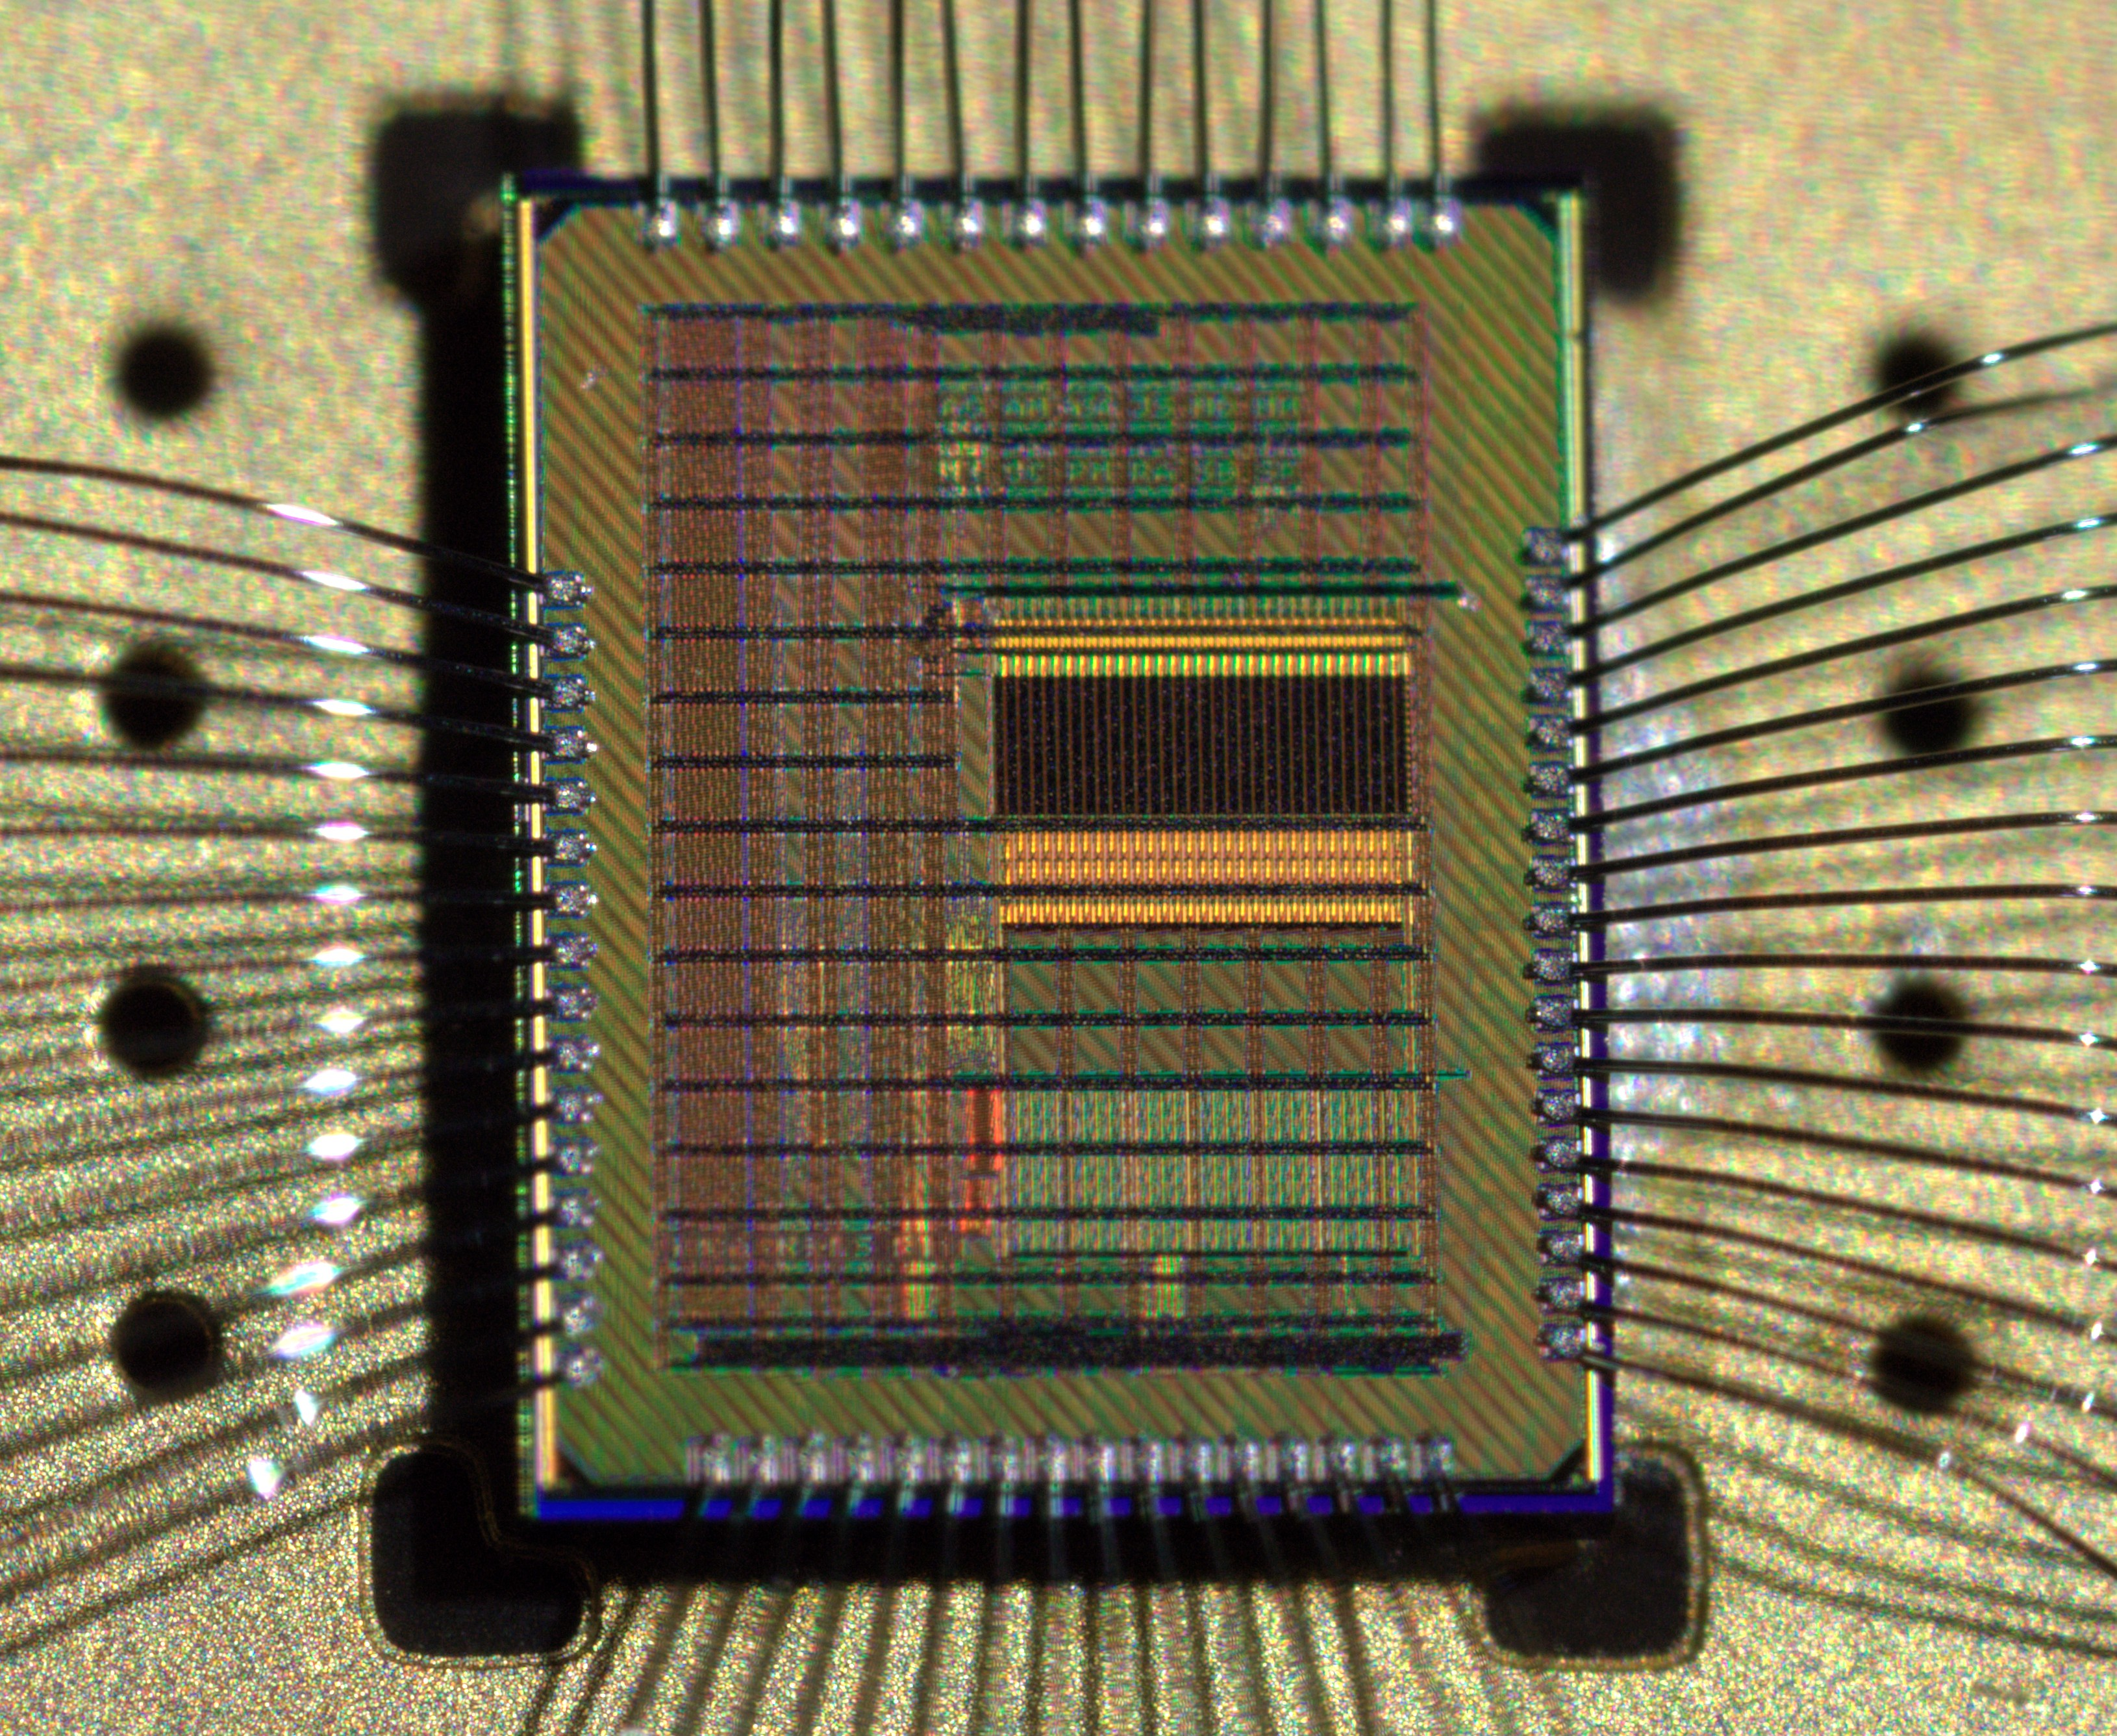
\includegraphics[width=\paperwidth]{pictures/dls_die_photo.jpg}};
}
\begin{frame}[plain]
\maketitle
\note{ Welcome everybody to this talk about my Bachelor thesis. As this is a quite technical talk, feel free to ask questions at any time.
The topic of my thesis was Extending Compiler Support for the BrainScaleS Plasticity Processor.}
\end{frame}

}

\begin{frame}{Contents}
\begin{columns}[c]
    \begin{column}{.5\textwidth}
        \begin{minipage}[t][0.5\textheight]{0.75\textwidth}
            \tableofcontents[sectionstyle=show, subsectionstyle=show/show/shaded]
        \end{minipage}\hfill
    \end{column}

    \begin{column}{.5\textwidth}
        \centering
        \begin{figure}
            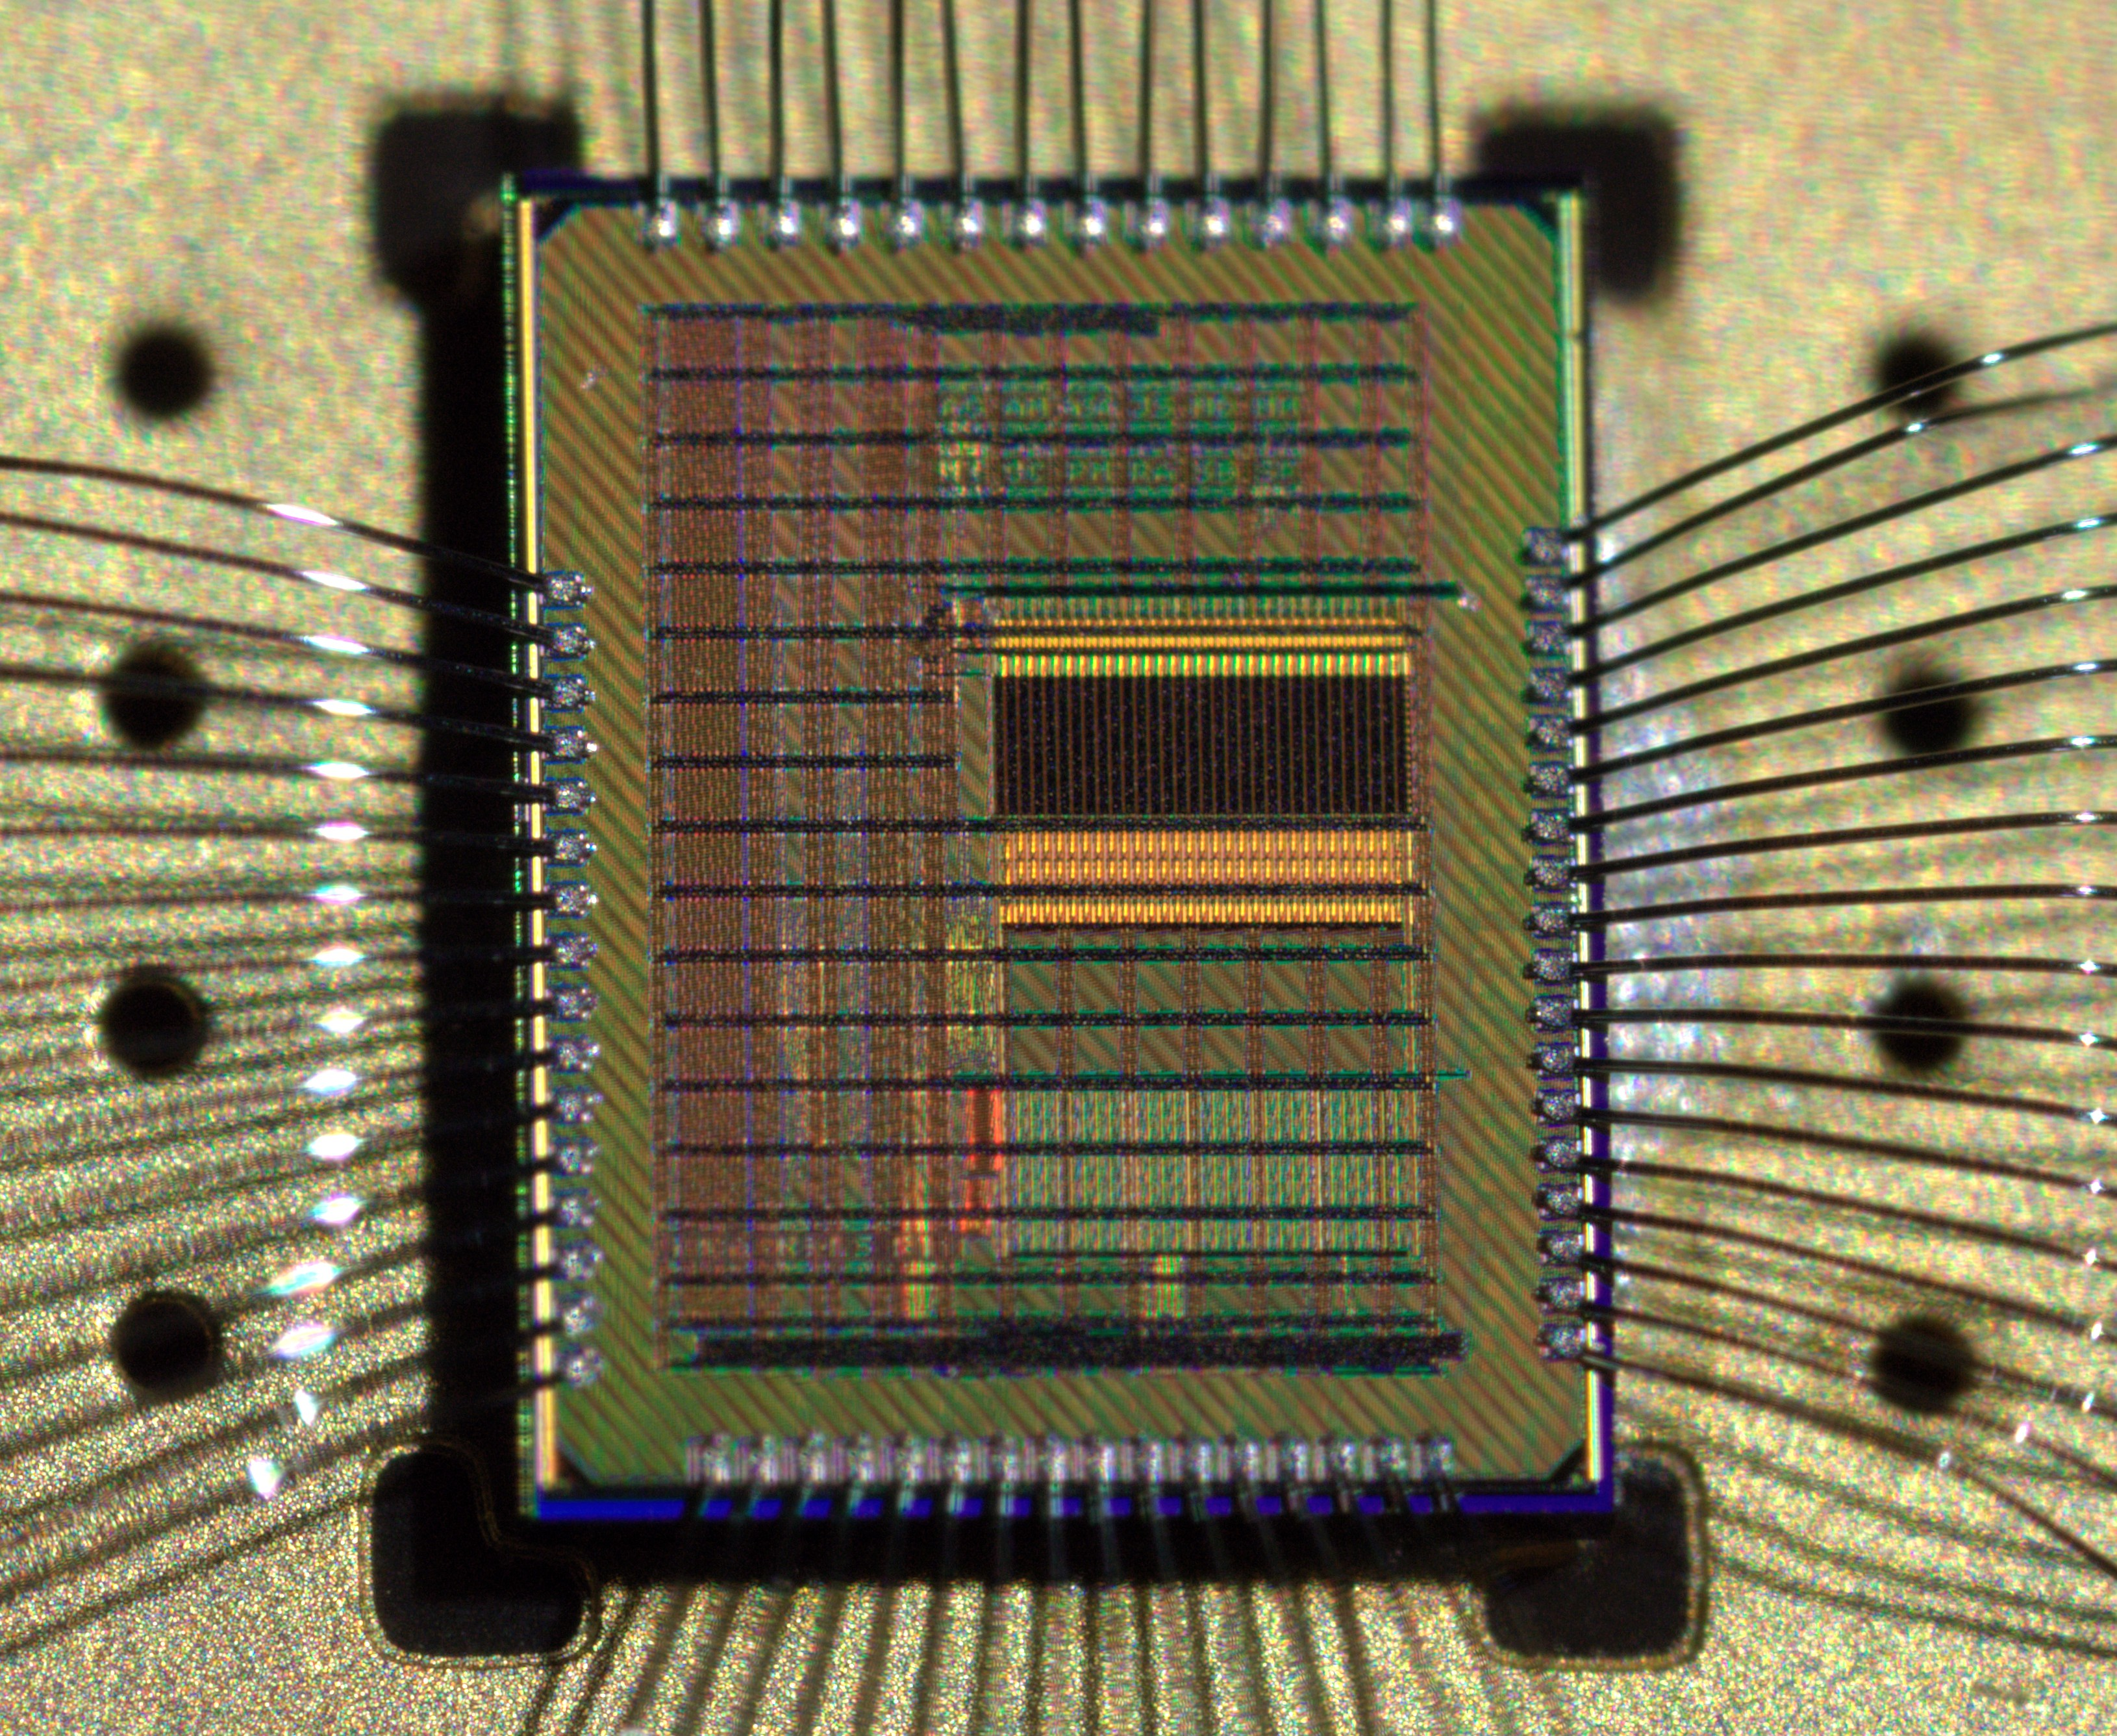
\includegraphics[width=\textwidth]{pictures/dls_die_photo.jpg}
            \caption{\label{fig:dls} Photograph of HICANN-DLS chip, \citeauthor{PPU}}
        \end{figure}
    \end{column}
\end{columns}
\note{
    as the title hints there are two main components to this talk, which are the plasticity processing unit (PPU) and Compilers.
    I will briefly talk about both of these and their applications.
    Afterwards I will explain, what I did during my thesis, which is of course followed by a short presentation of the results.

    But first I should explain, what the PPU is.
}
\end{frame}

% sections in the presentation
\section{PPU Architecture}
\begin{frame}{HICANN-DLS}
    \begin{columns}[c]
    \begin{column}{0.5\textwidth}
        \centering
        \begin{figure}
                \begin{adjustbox}{center, max width={.40\columnwidth}}
                    
\noindent{\begin{minipage}{\textwidth}
   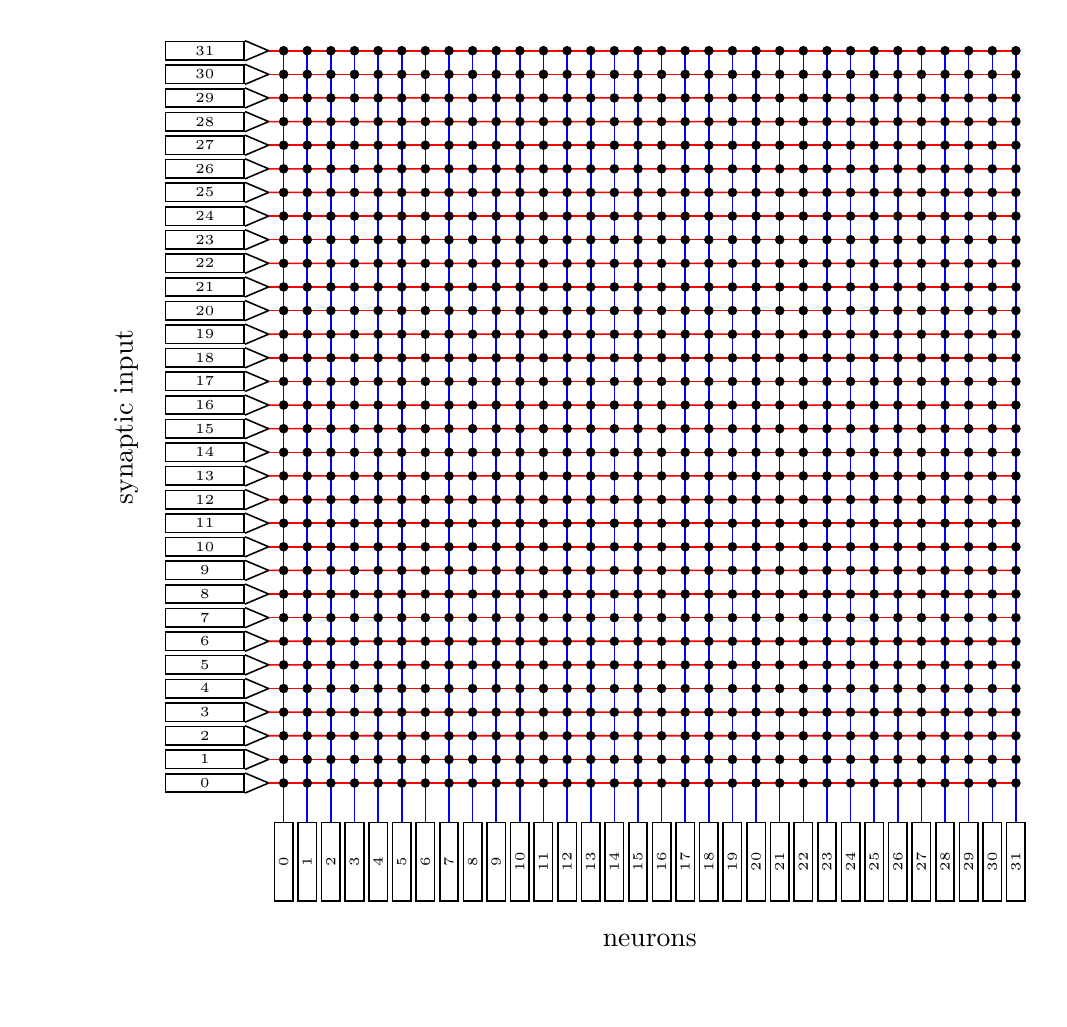
\begin{tikzpicture}[style={circle,draw,fill=black,minimum size=15}, line width=.2mm,
            vblock/.style={
            draw,
            fill=white,
            rectangle,
            minimum width=1.0cm,
            minimum height=0.3,
            font=\tiny},
            hblock/.style={
            draw,
            fill=white,
            rectangle,
            minimum width=.3,
            minimum height=1.0cm,
            font=\tiny}]

           \foreach \y in {0,...,31} 
           {
                      \node(domain)[vblock] (inrec\y) at (0, 0.3*\y + 1) {}; 
                      \draw[-] (inrec\y.north east) -- ($(inrec\y.north east)!.5!(inrec\y.south east)+(0.3,0)$) -- (inrec\y.south east);
                      \node (in\y) at (0, 0.3*\y + 1) {\tiny \y}; 
                      \draw[-, red] ($(inrec\y.north east)!.5!(inrec\y.south east)+(0.3,0)$) -- (0.3*31 + 1,0.3*\y + 1);
                  }
       \foreach \x in {0,...,31}
       { 
           \node(domain)[hblock] (neurec\x) at (0.3*\x + 1, 0) {}; 
           \node[rotate=90,] (neu\x) at (0.3*\x + 1, 0) {\tiny \x}; 
           \draw[-, blue] (neurec\x.north) -- (0.3*\x + 1,0.3*31 + 1);
           \foreach \y in {0,...,31} 
                  {\pgfmathtruncatemacro{\vlabel}{\y}
                  \draw [black,fill=black,radius=0.5mm, minimum size=0]  (0.3*\x + 1,0.3*\y + 1) circle;}
              }

              \node[rotate=90] (input) at (-1, 0.3*31/2 + 1) {synaptic input};
              \node[] (input) at (0.3*31/2 + 1, -1) {neurons};
   \end{tikzpicture}
\end{minipage}}

                \end{adjustbox}
            \caption{\label{fig:array} Schematic Representation of the Synapse Array on HICANN-DLS}
        \end{figure}

    \end{column}

    \begin{column}{0.5\textwidth}
        \centering
        \begin{figure}
            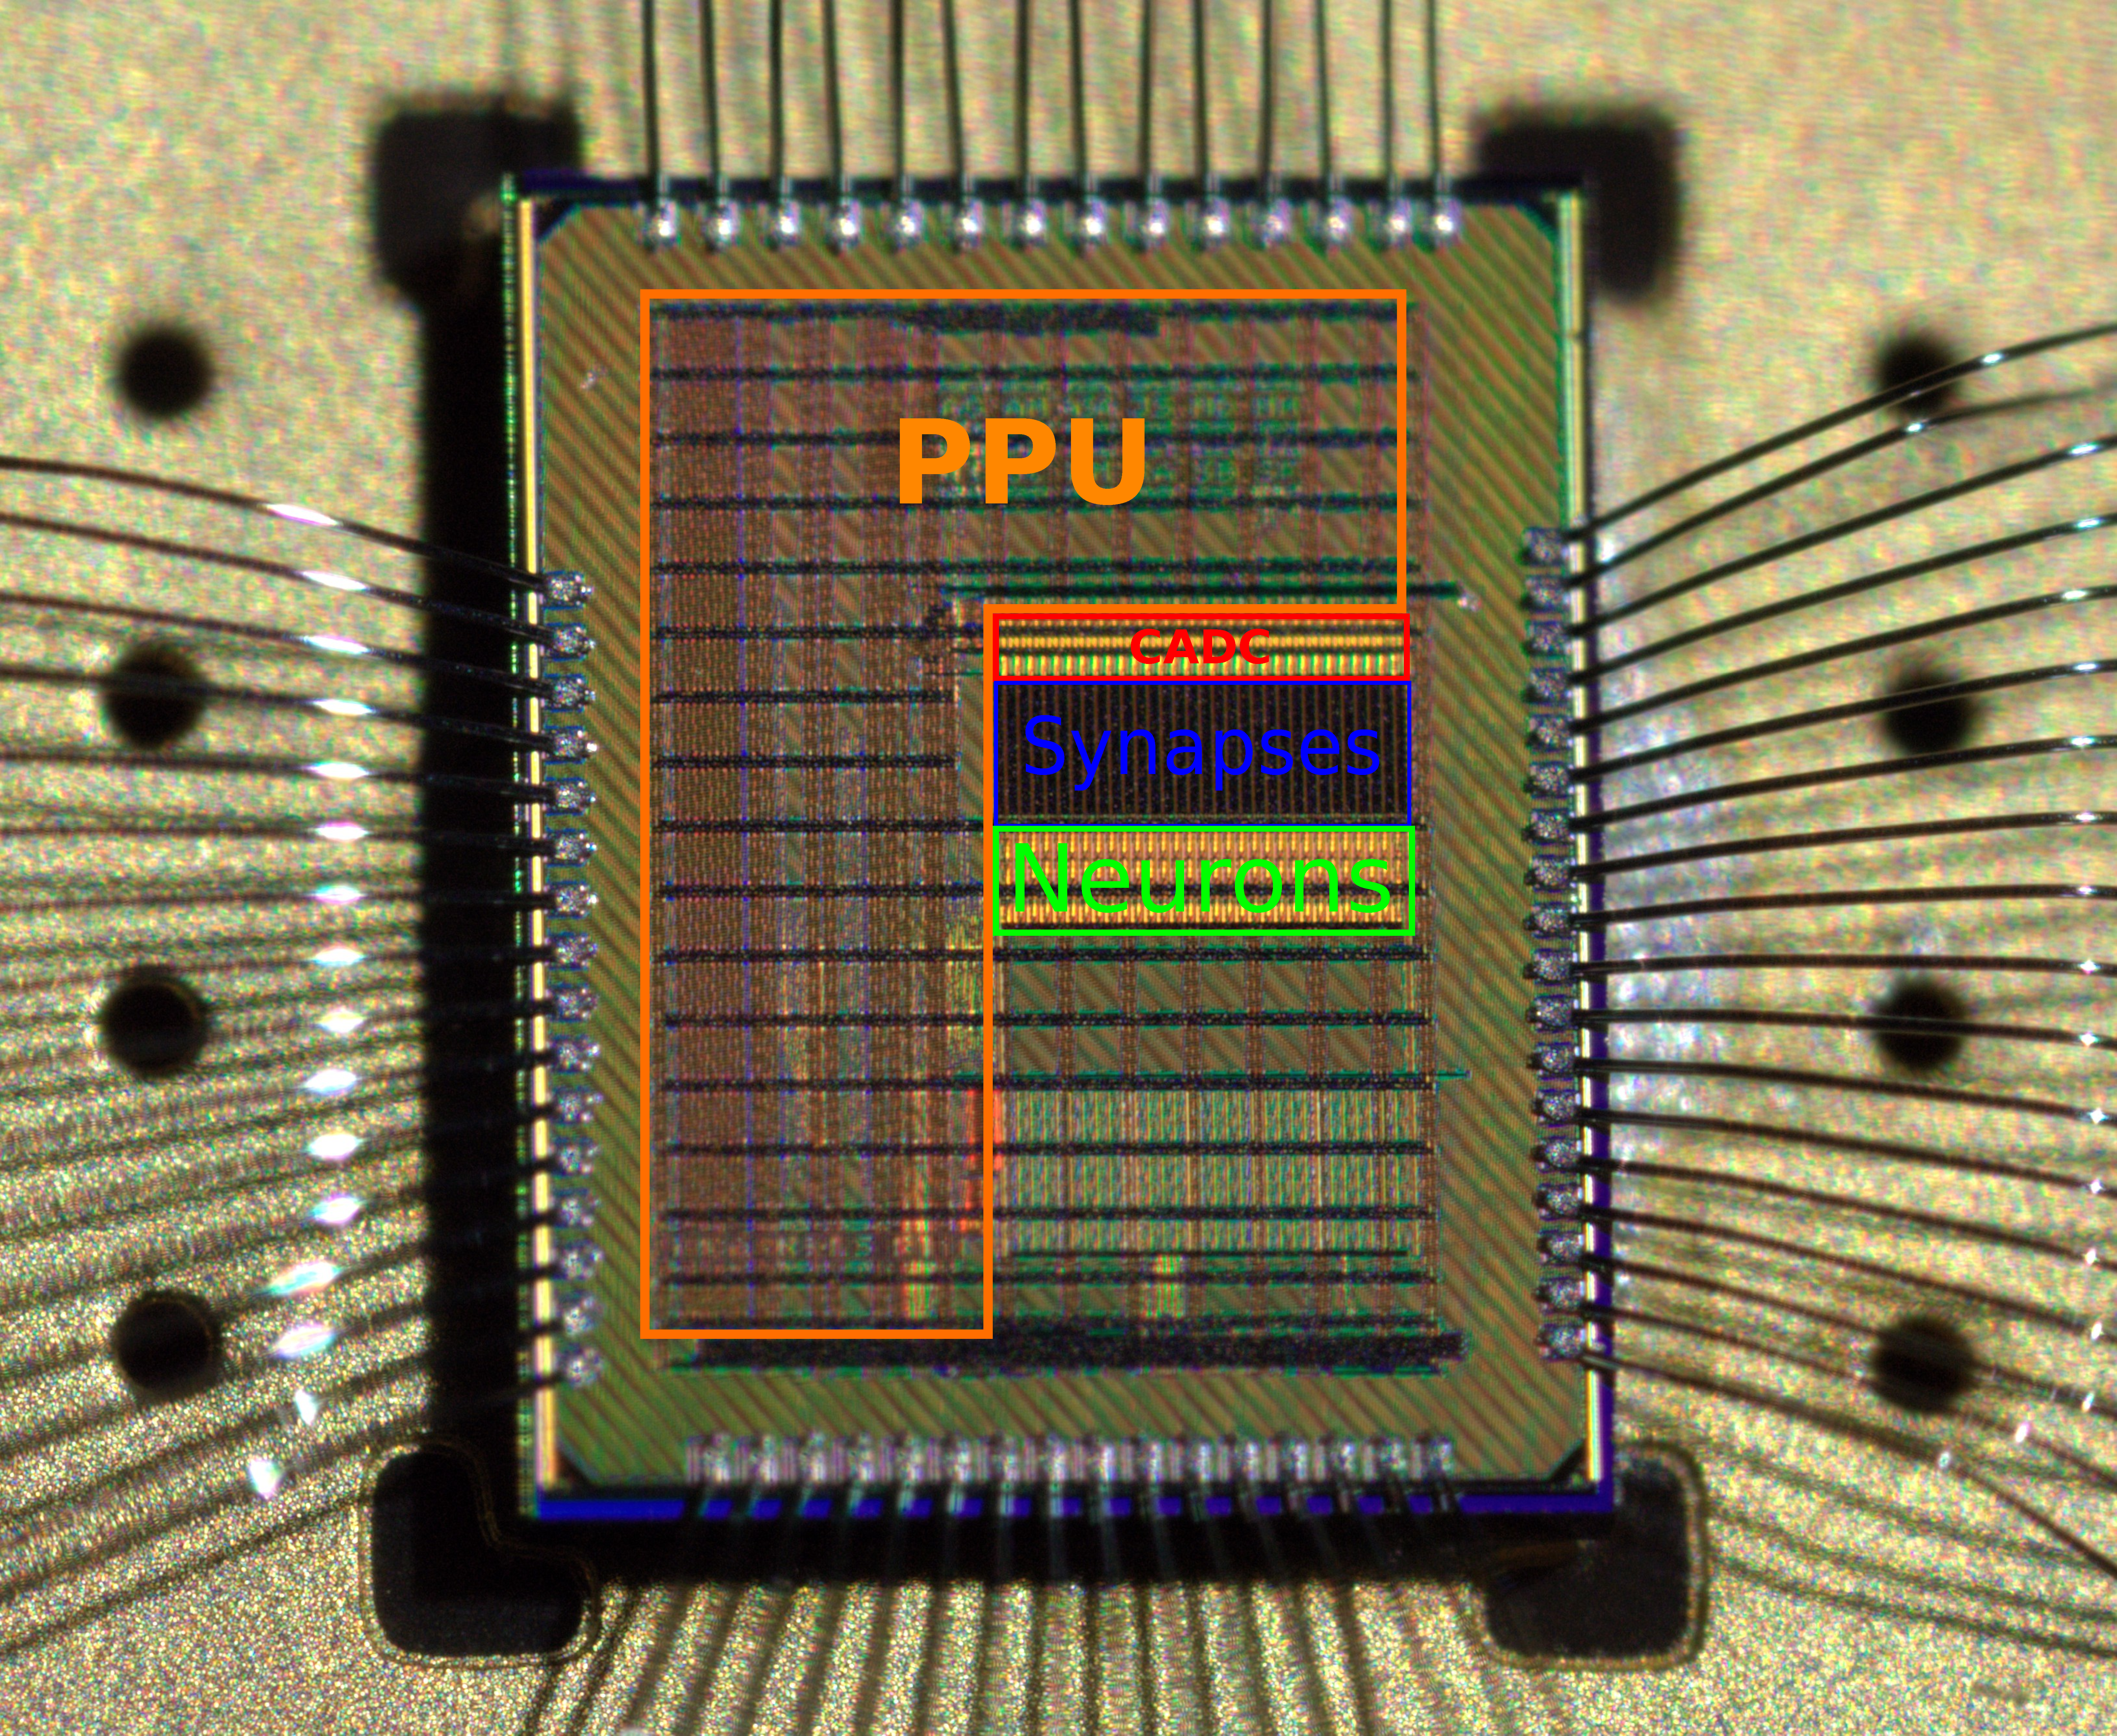
\includegraphics[width=\textwidth]{pictures/dls_marked.pdf}
            \caption{\label{fig:dls} Photograph of the HICANN-DLS Chip, modified from \citeauthor{PPU}}
        \end{figure}
    \end{column}
    \note{\tiny
        I am assuming that everybody here probably has heard about the HICANN-DLS.
        In short it is a chip that emulates neural networks through neurons and synapses that are implemented directly on the chip.
        What is special about the DLS, is the addition of a PPU to the HICANN.
        It is capable of performing simple computation and allows for on-line plasticity directly on the chip.

        As you can see to the right I have added a picture of the HICANN chip and marked the physical compartments.
        The PPU actually takes up a large space on the chip but before I am going to talk about the PPU, I will talk about the other parts briefly
        First we have the neurons.
        There are 32 neurons on the HICANN-DLS and each neuron is a circuit that receives some input signal which can cause the neurons to spike.
        These signals come from the so called synapse array.
        It connects 32 pre-synaptic inputs to all 32 neurons.
        This gives a total of 1024 synapses on each HICANN.
        
        Each synapse is realized through a circuit that takes the input signal and modifies it with a synpatic weight, that is saved in each synapse.
        There are also other properties to each synapse, but for this presentation it is enough to focus on the synaptic weights.
        Each synaptic weight is 6 bits wide, which is equivalent to numbers between 0 and 63 or a fixed-point number with an accuracy of $2^{-6}$.
		<bild whiteboard>
        Normally data segments are 8 bits wide, which is a byte, and the  superfluous bits are used for calibration of the synapse.
        
        The pre-synaptic inputs are handled by an FPGA, that takes care of spike routing.
        
        But there is also a correlation analog digital converter, that receives also signals of synapses if the forward signals to neurons.
        Through the CADC one can read out correlation that can be used for plasticity.

        The PPU is this remaining large section of the HICANN chip.
		This mostly is an existing architecture, that is called POWER architecture, which was extended with a custom vector extension which we will call s2pp.

		In general it is good to keep this in mind during this talk:
		The processing unit in HICANN DLS is called the PPU, the architecture with the vector extension is called nux architecture and the vector extension will be called s2pp.

}
    \end{columns}
\end{frame}

\begin{frame}{Plasticity Processing Unit}
    \begin{columns}[c]
    \begin{column}{0.5\textwidth}
        \begin{itemize}
			\setlength\itemsep{1em}
            \item ``Common'' von-Neumann architecture
			\item Machine Instructions
            \item Arithmetic Logic Unit (ALU)
            \item $\textrm{latency}(\textrm{register}) \ll \textrm{latency}(\textrm{memory}) $
		\end{itemize}
    \end{column}

    \begin{column}{0.5\textwidth}
        \centering
        \vspace*{3em}
        \begin{figure}
                \begin{adjustbox}{center, max width={.7\columnwidth}}
                    \tcbset
{enhanced,colframe=blue!70!black,colback=white!50!blue,colupper=red!50!black,
fonttitle=\bfseries,center title, size=small}

\centering

%\begin{tcolorbox}[enhanced jigsaw, width=\linewidth, remember as=pp, opacityframe=0.0, opacityback=0.0, nobeforeafter]
\tcbset
{enhanced,colframe=blue!70!black,colback=white!50!blue,colupper=red!50!black,
fonttitle=\bfseries,nobeforeafter,center title, noparskip, size=small}

\begin{tikzpicture}[line width=1mm]
    
    \node[] (c) at (0,0) {
    \begin{tcolorbox}[width=.65\linewidth, enhanced jigsaw, remember as=cpu, size=normal]
        \centering
        Processor
    
        \begin{tcolorbox}[enhanced jigsaw, noparskip,opacityframe=0.3, opacityback=0.3, width=\linewidth, height=.7cm, size=small, remember as=cs]
        \centering
        Control Section
        \end{tcolorbox}
    
        \begin{tcolorbox}[enhanced jigsaw, noparskip,opacityframe=0.3, opacityback=0.3, width=\linewidth, size=small, fontupper=\footnotesize]
            \centering
    
            \begin{tcolorbox}[enhanced, width=\linewidth, remember as=alu]
                \centering
                ALU
            \end{tcolorbox}
            \begin{tcolorbox}[enhanced, width=\linewidth, remember as=rf]
                \centering
                Register File
            \end{tcolorbox}
    
            Operational Section
        \end{tcolorbox}
    
    \end{tcolorbox}
    };
    \end{tikzpicture}
    
\begin{tikzpicture}[overlay,remember picture,line width=0.5mm]
    
    \node[] (a) at ($(cs.west)!.0!(cs.north west)-(1.5,0)$) {
        \begin{tcolorbox}[enhanced jigsaw, opacityframe=0.3, opacityback=0.3, height=0.7cm, width=.15\linewidth, remember as=in, watermark text=Input, nobeforeafter]
        \end{tcolorbox}
    };
    
    \node[] (b) at ($(cs.east)!.0!(cs.north east)+(1.5,0)$) {
    \begin{tcolorbox}[enhanced jigsaw, opacityframe=0.3, opacityback=0.3, height=0.7cm, width=.15\linewidth, remember as=out, watermark text=Output, nobeforeafter]
    \end{tcolorbox}
    };
    
    \draw[->, shorten >=-1.0mm] (in.east) -- ($(cs.west)!.0!(cs.north west)$);
    \draw[->, shorten >=-1.0mm] ($(cs.east)!.0!(cs.north east)$) -- (out.west);

    \draw[->, shorten >=-1.0mm] ($(cs.west)!.5!(cs.south west)$) to [out=225, in=180] (alu.west);
    \draw[->, shorten >=-1.0mm] (alu.east) to [out=20, in=315] ($(cs.east)!.5!(cs.south east)$);
    
    \draw[->, shorten >=-1.0mm] ($(alu.south)!.5!(alu.south east)$) -- ($(rf.north)!.5!(rf.north east)$);
    \draw[->, shorten >=-1.0mm] ($(rf.north)!.5!(rf.north west)$) -- ($(alu.south)!.5!(alu.south west)$);
\end{tikzpicture}


% \begin{tikzpicture}[overlay,remember picture,line width=1mm]
%     \draw[->, shorten >=-1.5mm] ($(cp.north)+(0,1)$) -- (sc.north);
%     \draw[->, shorten >=-1.5mm] (sc.south) -- (ps.north);
%     \draw[->, shorten >=-1.5mm] (ps.south) -- (sa.north);
%     \draw[->, shorten >=-1.5mm] (sa.south) -- (sco.north);
%     \draw[-] (sco.south) -- (me.north);
%     \draw[->, shorten >=-1.5mm] (me.south) -- (cg.north);
%     \draw[->, shorten >=-1.5mm] (cg.south) -- (tco.north);
%     \draw[->] (tco.south) -- ($(cp.south)+(0,-1)$);
% \end{tikzpicture}
% \begin{tikzpicture}[overlay,remember picture,line width=1mm]
%     \draw[-, draw=blue!30!white,line width=.5mm, shorten >=.2cm,shorten <=.1cm] (cmp.north east) -- (cp.north west);
%     \draw[-, draw=blue!30!white,line width=.5mm, shorten >=.2cm,shorten <=.1cm] (cmp.south east) -- (cp.south west);
% \end{tikzpicture}

                \end{adjustbox}
            \caption{\label{fig:processor} Schematic of General Purpose Processor with von-Neumann Architecture}
        \end{figure}
    \end{column}
    \end{columns}
\note{	But before I shall go into more detail, I have to talk about processors in general.
		As you may know, next to all computing nowadays is done by processors which are often described as CPUs.
		The processors are normally built according to the von-Neumann architecture, which combines programs and data in the same memory.
		The processor fetches instructions from the memory and analyzes them to decide what to do.
		Most instructions get passed to the ALU that performs any sort of computation in the processor.
		To do this, the ALU has access to so called registers.
		These registers can hold small amounts of data but offer a very low access time.
		The ALU uses these registers for computation and saves results there as well.
		Data is then written separately into memory or new values for registers are loaded from memory.
		This usually takes a significant amount of time longer than access to registers and thus, programs try to use registers as much as possible.
}

\end{frame}

\begin{frame}{PPU Architecture}
    \begin{columns}[c]
    \begin{column}{0.5\textwidth}
        \begin{itemize}
			\setlength\itemsep{1em}
			\item Based on POWER architecture
            \item Vector Extension \\ \hspace{10mm}
				$\rightarrow$ Parallelization \\ \hspace{10mm}
				$\rightarrow$ Performance
            \item Weight Updates
			\item Access to Synaptic Array
        \end{itemize}
    \end{column}

    \begin{column}{0.5\textwidth}
        \centering
        \begin{figure}
            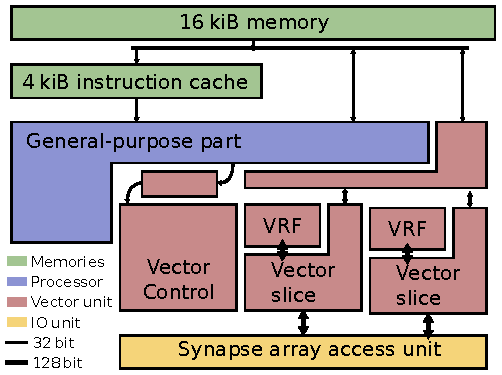
\includegraphics[width=.8\textwidth]{pictures/nux.pdf}
            \caption{\label{fig:nux} Structure of nux Architecture}
        \end{figure}
    \end{column}
    \end{columns}
\note{	
		Instead of the ALU, some instructions can be passed to other units that can perform special instructions.
		These units may also use different registers.

		This is the case for the PPU.
		It includes a special vector extension that includes vector registers as well.
		Using vector registers is favorable for operations that use have to be applied to multiple values and can be done in parallel.
		
		This is the strength of the PPU as is allows to compute weight updates of up to 16 synapses at the same time, which increases performance significantly. 
		For this reason the PPU is also connected to the synaptic array and is able to read out and write synaptic weights.
		Although it induces a problem because the vector unit uses special instructions that are unique to the nux architecture.
}
\end{frame}



\section{GCC Structure}
\begin{frame}[fragile]{Compiler Structure}
    \begin{columns}[c]
    \begin{column}{0.5\textwidth}
        \begin{itemize}
			\setlength\itemsep{1em}
            \item Program $\xrightarrow{\text{compile}}$ Executable
			\item Compiling Stages
			\item Compiler $\rightarrow$ Assembly
			\item Back-End is target-dependent
        \end{itemize}
    \end{column}

    \begin{column}{0.5\textwidth}
        \centering
        \begin{figure}
            \begin{adjustbox}{center, max width={.5\columnwidth}}
                    \tcbset
    {my box/.style={enhanced,colframe=blue!70!black,colback=white!50!blue,colupper=red!50!black,
        fonttitle=\bfseries,nobeforeafter,center title, noparskip, size=small},
    every box on layer 1/.style={every box},
    every box on layer 2/.style={reset,my box}}
\begin{tcolorbox}[enhanced jigsaw, width=\textwidth, opacityframe=0.0, opacityback=0.0]
\begin{tcolorbox}[enhanced, height=.5cm, width=\linewidth, remember as=pp, opacityframe=0.0, opacityback=0.0]\end{tcolorbox}
\begin{tcolorbox}[enhanced, height=.7cm, width=\linewidth, watermark text=Preprocessor, remember as=pp]\end{tcolorbox}
\begin{tcolorbox}[tcbox raise base, width=\linewidth, enhanced jigsaw, remember as=cmp]
    \begin{tcolorbox}[enhanced, breakable, noparskip,opacityframe=0.3, opacityback=0.3, height=1.4cm, width=\linewidth, watermark text=Front-End, remember as=fe]
    \end{tcolorbox}
    \begin{tcolorbox}[enhanced, breakable, noparskip,opacityframe=0.3, opacityback=0.3, height=0.7cm, width=\linewidth, watermark text=Middle-End, remember as=me]
    \end{tcolorbox}
    \begin{tcolorbox}[enhanced, breakable, noparskip,opacityframe=0.3, opacityback=0.3, height=1.1cm, width=\linewidth, watermark text=Back-End, remember as=be]
    \end{tcolorbox}
\end{tcolorbox}

\end{tcolorbox}

\begin{tikzpicture}[overlay,remember picture,line width=1mm]
    \draw[->, shorten >=-1.5mm] ($(pp.north)+(0,1.5)$) -- node [left] {program code} (pp.north);
    \draw[->, shorten >=-1.5mm] (pp.south) -- (fe.north);
    \draw[->, shorten >=-1.5mm] (fe.south) -- (me.north);
    \draw[->, shorten >=-1.5mm] (me.south) -- (be.north);
    \draw[->] (be.south) -- node [left] {machine files} ++(0,-1.5);
\end{tikzpicture}

                    \tcbset
    {my box/.style={enhanced,colframe=blue!70!black,colback=white!50!blue,colupper=red!50!black,
        fonttitle=\bfseries,nobeforeafter,center title, noparskip, size=small},
    every box on layer 1/.style={every box},
    every box on layer 2/.style={reset,my box}}
\begin{tcolorbox}[enhanced jigsaw, width=\linewidth, remember as=pp, opacityframe=0.0, opacityback=0.0]
\begin{tcolorbox}[tcbox raise base, width=\linewidth, enhanced jigsaw, remember as=cp]
    \begin{tcolorbox}[enhanced jigsaw, breakable, noparskip,opacityframe=0.3, opacityback=0.3, width=\linewidth, size=small]
        \begin{tcolorbox}[enhanced,center title,width=\linewidth, remember as=sc, height=0.7cm,top=1mm,bottom=1mm]
            \begin{center}Scanner\end{center}
        \end{tcolorbox}
        \begin{tcolorbox}[enhanced,width=\linewidth, remember as=ps,top=1mm,bottom=1mm]
            \begin{center}Parser\end{center}  
        \end{tcolorbox}
        \begin{tcolorbox}[enhanced, width=\linewidth, remember as=sa,top=1mm,bottom=1mm]
            \begin{center}Semantic Analyzer \end{center} 
        \end{tcolorbox}
        \begin{tcolorbox}[enhanced, width=\linewidth, remember as=sco,top=1mm,bottom=1mm]
            \begin{center}Source Code Optimizer \end{center}
        \end{tcolorbox}
    \end{tcolorbox}
    \begin{tcolorbox}[enhanced jigsaw, breakable, noparskip,opacityframe=0.3, opacityback=0.3, height=0.7cm, width=\linewidth, remember as=me, watermark text=Middle-End]
    \end{tcolorbox}
    \begin{tcolorbox}[enhanced jigsaw, breakable, noparskip,opacityframe=0.3, opacityback=0.3, width=\linewidth, size=small]
        \begin{tcolorbox}[enhanced, width=\linewidth, remember as=cg,top=1mm,bottom=1mm]
            \begin{center}Code Generator  \end{center}
        \end{tcolorbox}
        \begin{tcolorbox}[enhanced, width=\linewidth, remember as=tco,top=1mm,bottom=1mm]
            \begin{center}Target Code Optimizer \end{center}
        \end{tcolorbox}
    \end{tcolorbox}
\end{tcolorbox}
\end{tcolorbox}
\begin{tikzpicture}[overlay,remember picture,line width=1mm]
    \draw[->, shorten >=-1.5mm] ($(cp.north)+(0,1)$) -- (sc.north);
    \draw[->, shorten >=-1.5mm] (sc.south) -- (ps.north);
    \draw[->, shorten >=-1.5mm] (ps.south) -- (sa.north);
    \draw[->, shorten >=-1.5mm] (sa.south) -- (sco.north);
    \draw[-] (sco.south) -- (me.north);
    \draw[->, shorten >=-1.5mm] (me.south) -- (cg.north);
    \draw[->, shorten >=-1.5mm] (cg.south) -- (tco.north);
    \draw[->] (tco.south) -- ($(cp.south)+(0,-1)$);
\end{tikzpicture}
\begin{tikzpicture}[overlay,remember picture,line width=1mm]
    \draw[-, draw=blue!30!white,line width=.5mm, shorten >=.2cm,shorten <=.1cm] (cmp.north east) -- (cp.north west);
    \draw[-, draw=blue!30!white,line width=.5mm, shorten >=.2cm,shorten <=.1cm] (cmp.south east) -- (cp.south west);
\end{tikzpicture}

            \end{adjustbox}
            \caption{\label{fig:compiler} Structure of Compiling Process and Compiler}
        \end{figure}
    \end{column}
    \end{columns}
\note{	\scriptsize
		This is of special significance when using a compiler.
		But why?
		I am quite sure that all of you have used compilers just recently and generally know what they do.
		And most will probably say that a compiler compiles code, or to be more specific it converts a program into a file that the computer can run.
		This is of course right and is follows the definition of a compiler, but there is much more to it.
		
		What we usually call compiler consists of several stages that follow different purposes and like the preprocessor, that takes care of define instructions and substituting macros.
		The actual compiler will only take that preprocessed code and create an assembly file from this.
		Assembly is a language that consists of machine instructions which have specific names and represents pretty much the lowest level of coding a human would do.
		From there on the assembly file gets converted into a pure machine code, hence no names only numbers, file by the assembler and then is combined with other files and gets assigned a memory location by the linker and loader.
		
		But since I focused on the compiler in this thesis, I should also give an overview of the internal structure of a compiler.
		As you can see, this time there are different phases in the compiler and these similarly ordered like compiling stages.
		But we only need to focus on the last two stages which are part of the back-end.
		
		The back-end is mainly responsible for creating the actual machine code which was previously processed by the front-end and the middle-end.
		It then also optimizes the code it generated, but this is machine-dependent.
		In general a back-end is always machine-dependent as the assembly language is different for different processor architectures.
		One architecture, that most of you might know is the ARM architecture that is at the heart of every smartphone and also SpiNNaker.

	The PPU though, has a POWER architecture which is also called rs/6000.}
\end{frame}

\begin{frame}{GCC for the PPU}
    \begin{columns}[c]
    \begin{column}{0.5\textwidth}
        \begin{itemize}
			\setlength\itemsep{1em}
            \item No ``official'' support of s2pp
			\item Currently using macros
			\item Existing AltiVec extension
			\item Intrinsics $\rightarrow$ \textbf{use this}
        \end{itemize}
    \end{column}

    \begin{column}{0.5\textwidth}
        \centering
        \begin{figure}
            \begin{adjustbox}{center, max width={.5\columnwidth}}
                listing of PPU code
            \end{adjustbox}
            \caption{\label{fig:compiler} Structure of Compiling Process and Compiler}
        \end{figure}
    \end{column}
    \end{columns}
\note{\scriptsize	now there exist different compilers and the one which is used by this group is the GCC.
		GCC is a compiler that is wide-spread especially at academic institutions.
		it is capable of compiling for a large variety of languages and also most processor architectures there are.
		Unfortunately this does not include the nux architecture.
		Although the basic architecture of nux is supported, there is no official support of the vector extension.

		This means that users can code in C for example but every time they need to use the vector extension, it is necessary to handle assembly code.
		There have been efforts to make this easier, but still it mostly looks like this when programming for the PPU.
		<bild zeigen>
		Although there ARE ways to program vector extensions that look more common.
	
		One such extension is the AltiVec extension to the POWER architecture.
		So in a way this is a competing vector extension to s2pp and programming for AltiVec usually looks like this.

		it uses so called intrinsics for vector processing.
		An intrinsic basically works like a function, the same way addition is also a function, only does it map on a specific machine instruction that is invoked when using an intrinsic.

		And if we compare these two, I think it becomes clear that this is what we want.
}
\end{frame}


\section{Extending GCC for the PPU}
\begin{frame}{Main Work of this Thesis}
    \begin{columns}[c]
    \begin{column}{0.5\textwidth}
        \begin{itemize}
			\setlength\itemsep{1em}
            \item No ``official'' support of s2pp
			\item Currently using macros
			\item Existing AltiVec extension
			\item Intrinsics $\rightarrow$ \textbf{use this}
        \end{itemize}
    \end{column}

    \begin{column}{0.5\textwidth}
        \centering
        \begin{figure}
            \begin{adjustbox}{center, max width={.5\columnwidth}}
                listing of PPU code
            \end{adjustbox}
            \caption{\label{fig:compiler} Structure of Compiling Process and Compiler}
        \end{figure}
    \end{column}
    \end{columns}
\note{	And this is what I did throughout my Bachelor's thesis.
		I added support for the nux architecture by extending the GCC back-end for POWER.
		And as simple as sounds it was quite a challenge, since there was no documentation but comments and general information on how to create a back-end.

		Luckily there is already the AltiVec extension which I mentioned earlier and it provided a good guideline for me to find relevant sections in code.

		Ultimately I had to go through roughly 50.000 lines of code and it needed about 3.000 additional lines to add support for the s2pp vector extension.

		Now I want to show you the results of this and also give an outlook, of what might be possible in the future.
}
\end{frame}

\section{Results}
\begin{frame}[fragile]{New Features}
    \begin{columns}[c]
    \begin{column}{0.5\textwidth}
        \begin{itemize}
			\setlength\itemsep{1em}
            \item |-mcpu=nux| target flag
			\item |vector| attribute
			\item s2pp vector intrinsics
			\item Inline assembly
			\item Supports optimization
        \end{itemize}
    \end{column}

    \begin{column}{0.5\textwidth}
        \centering
        \begin{figure}
            \begin{adjustbox}{center, max width={.5\columnwidth}}
                listing of PPU code
            \end{adjustbox}
            \caption{\label{fig:compiler} Structure of Compiling Process and Compiler}
        \end{figure}
    \end{column}
    \end{columns}
\note{	Let's start with generating code for the PPU.
		It simply takes one target flag and a header file, to create code for the complete nux architecture.
		<bild>
		Also there is a vector type which can be used to represent vectors as variables and it works exactly like other existing vector attributes.
		<extend picture>
		Most importantly, users can now use intrinsics for simple vector instructions and use the vector variables instead of arbitrary macros.
		<extend picture>
		Furthermore, there is inline assembly support which allows for simpler low level coding whenever it is needed.
		<extend picture>
		And all of this also supports optimization, that allows for efficient programs on the PPU, without particular knowledge by the user.
		<beispiel mit und ohne optimiereung>	
}
\end{frame}

\begin{frame}[fragile]{Outlook}
    \begin{columns}[c]
    \begin{column}{0.5\textwidth}
        \begin{itemize}
			\setlength\itemsep{1em}
			\item Further testing for bugs
			\item Existing applications with |libnux|
			\item Extending test coverage
			\item Debugging support?
			\item \textbf{New tool for development!}
        \end{itemize}
    \end{column}

    \begin{column}{0.5\textwidth}
        \centering
        \begin{figure}
            \begin{adjustbox}{center, max width={.5\columnwidth}}
                listing of PPU code
            \end{adjustbox}
            \caption{\label{fig:compiler} Structure of Compiling Process and Compiler}
        \end{figure}
    \end{column}
    \end{columns}
\note{	\scriptsize
		Of course I have to mention that this is kind of a beta phase and that there are bugs that can occur.
		But the more people will use this compiler, the more bugs can be fixed and this will become an even more handy tool, when programming for the PPU.
		
		Nonetheless there already exist programs and tests that make use of the compiler extension.

		This for example is the program David Stöckel used for his criticality tests, which he presented a few weeks ago.
		You can see the use of a testing framework which David established, called libnux.
		This is also a great help when programming for the PPU since it is available.

		And this is one of a few tests which later shall extend the exiting testing scenarios on the PPU.

		And there is more of what might be possible in the future with compiler support of nux.
		For once it will be easier to create high-level tests for the PPU and extending the current test coverage is something I would like to do in the future.
		Also it might be possible to realize GDB support for the PPU, which would allow for extended debugging of PPU software but this is something that is not yet on the agenda.

		All in all I want to encourage as many of you as possible to use the new compiler, as it will become better over time as more users develop with it.
		And I hope, that I was able to give a comprehensive introduction to the compiler and some fundamentals of processor architecture.

		If by any means some of you are interested in learning more about these topics I recommend the following books, which helped me to get into the subject and which I also used for references.
		
}
\end{frame}

\appendix

\section{Appendix}
\scriptsize
\nocite{microprocessor}
\nocite{UBHD-67548259}
\nocite{UBHD-66483012}
\nocite{nuxmanual}
\nocite{GCCint}
\begin{frame}[fragile]{References}
\bibliographystyle{bib/agu}
\bibliography{bib/myrefs}
\note{	thank you all for listening to this rather technical talk.
}
\end{frame}

\begin{frame}[fragile]{Whiteboard}
\begin{columns}[c]
	\begin{column}{.5\textwidth}
\begin{figure}[htpb]
    \centering
		\scriptsize
        \begin{bytefield}[bitwidth=0.11111111\textwidth, bitheight=2em]{8}
            \bitheader[endianness=big]{0-7}\\
            \bitbox{1}{\color{lightgray}\rule{\width}{\height}} & \bitbox{1}{\color{lightgray}\rule{\width}{\height}} & \bitbox{1}{$2^{-1}$} & \bitbox{1}{$2^{-2}$} & \bitbox{1}{$2^{-3}$} & \bitbox{1}{$2^{-4}$} & \bitbox{1}{$2^{-5}$} & \bitbox{1}{$2^{-6}$}\\
        \end{bytefield}
        \begin{bytefield}[bitwidth=0.11111111\textwidth, bitheight=2em]{8}
            \bitheader[endianness=big]{0-7}\\
            \bitbox{1}{$-1$} & \bitbox{1}{$2^{-1}$} & \bitbox{1}{$2^{-2}$} & \bitbox{1}{$2^{-3}$} & \bitbox{1}{$2^{-4}$} & \bitbox{1}{$2^{-5}$} & \bitbox{1}{$2^{-5}$} & \bitbox{1}{$2^{-7}$}\\
        \end{bytefield}
    \caption{\label{fig:fractional} Comparison of the Representation of Weights in Synapses and the Fractional Representation of Vector Components for Fixed-Point Saturational Arithmetic}
\end{figure}
\end{column}
	\begin{column}{.5\textwidth}
\begin{description}
    \item[PPU] is the processor which is part of HICANN-DLS and mainly responsible for plasticity.
    \item[nux] refers to the architecture of the PPU, see figure.
    \item[s2pp] describes the PPU's VE and is part of the nux architecture.
\end{description}
	\end{column}
\end{columns}
\end{frame}

\scriptsize

\begin{frame}[fragile]{Additional Figures}
	\vspace*{2em}
	\begin{columns}[t]
		\begin{column}{.5\textwidth}
\begin{figure}
    \centering
    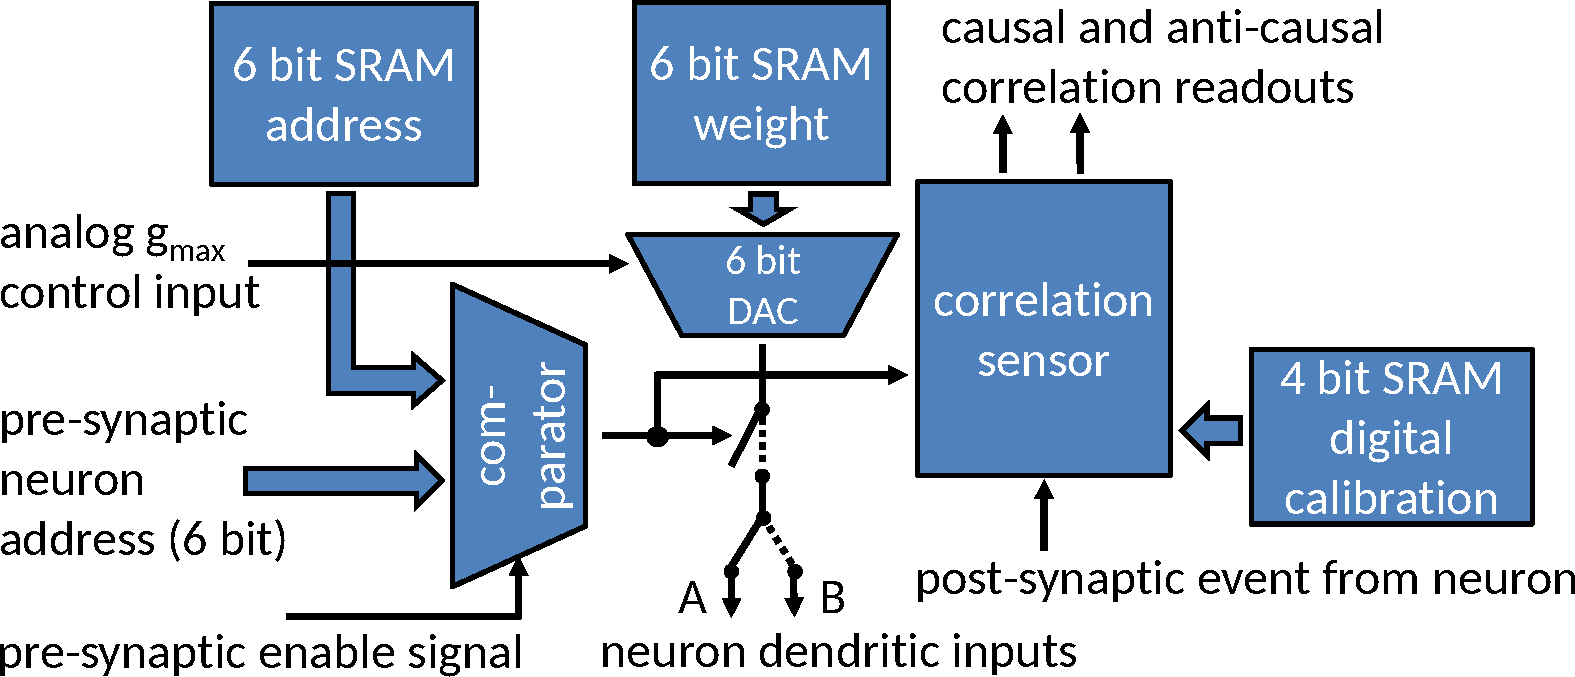
\includegraphics[width=\textwidth]{pictures/syncircuit.pdf}
    \caption{\label{fig:circuit} Block Diagram of the Synapse Circuit (modified from~\citeauthor{PPU}).}
\end{figure}
	\vspace*{-1em}
\begin{figure}
    \centering
    \begin{bytefield}[endianness=big, bitwidth=0.027777\linewidth, bitheight=2em]{32}
        \bitheader{0,7,15,23,31}\\
        \bitboxes{8}{{mnemonic}{operand}{operand}{operand}}\\
        \bitboxes{8}{{\tt{addi}}{{\tt r1} \\ \tiny register address}{{\tt r2} \\ \tiny register address}{{\tt 5} \\ \tiny immediate operand}}
    \end{bytefield}
    \caption{\label{fig:mnemonic} Representation of Assembly Instruction {\tt addi} as a Machine Instruction in Memory. The immediate value {\tt 5} is added to register {\tt r2} and the result written in {\tt r1}.}
\end{figure}

		\end{column}
		\begin{column}{.5\textwidth}

\begin{figure}
    \centering
    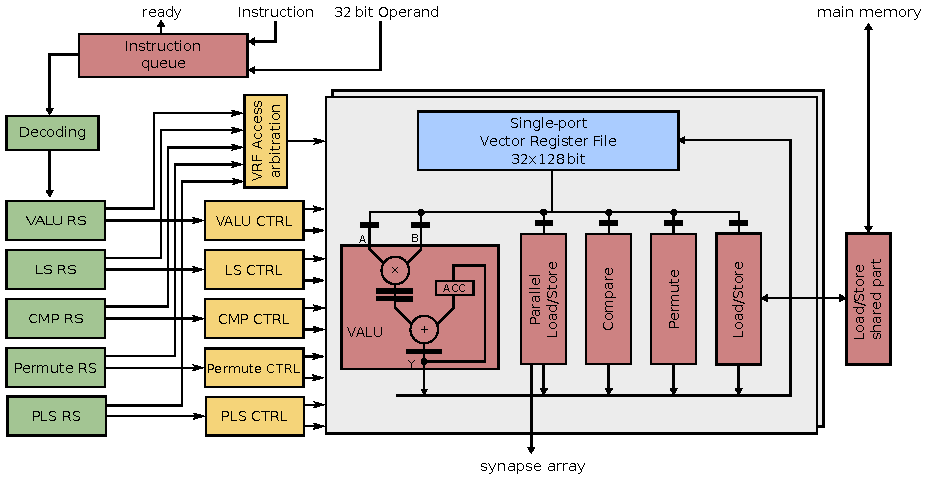
\includegraphics[width=\textwidth]{pictures/s2pp.pdf}
    \caption{\label{fig:s2pp} Detailed Structure of the s2pp Vector Extension (taken from~\citeauthor{PPU})}
\end{figure}
		\end{column}
	\end{columns}

\end{frame}
\begin{frame}[fragile]{Additional Figures}

\begin{figure}
	\vspace*{3em}
    \centering
	\begin{bytefield}[endianness=little, bitwidth=\widthof{\tiny bit}/2, bitheight=2em]{128}
        \bitheader{0,7,15,31,63,127}\\
    \bitboxes{8}{{QI}{\tiny Quarter \\ Integer}{}{}{}{}{}{}{}{}{}{}{}{}{}{}}\\
    \bitboxes{16}{{HI}{\tiny Half \\ Integer}{}{}{}{}{}{}}\\
	\bitboxes{32}{{SI}{\tiny Single \\ Integer}{}{}}\\
    \bitboxes{32}{{SF}{\tiny Single \\ Float}{}{}}\\
    \end{bytefield}
	\vspace*{-1.5em}
    \caption{\label{fig:vectorlength} Vector structures are 128 bits wide and split into common word sizes.}
\end{figure}

\begin{figure}
	\begin{bytefield}[endianness=little, bitheight=2em, bitwidth=\widthof{\tiny bit}]{32}
        \bitheader{0,1,7,15,31}\\
        \colorbitbox{lightgray}{1}{\tiny bit} && \bitbox{31}{}\\
        \colorbitbox{lightgray}{8}{byte} && \bitbox{24}{}\\
        \colorbitbox{lightgray}{16}{halfword} && \bitbox{16}{}\\
        \colorbitbox{lightgray}{32}{word}\\
    \end{bytefield}
	\vspace*{-1.5em}
    \caption{\label{fig:bitlength} Illustration of Word Sizes for 32-bit Words}
\end{figure}

\end{frame}

\end{document}
